\section{Liste der Parks}
\label{parklist}

Diese View gibt Auskunft über alle Parks, welche sich auf dem Server befinden. Hier befinden sich die 
Namen, die durchschnittliche Bewertungen und die Bilder aller Parks. 

\begin{figure}[H]
    \begin{center}
      \frame{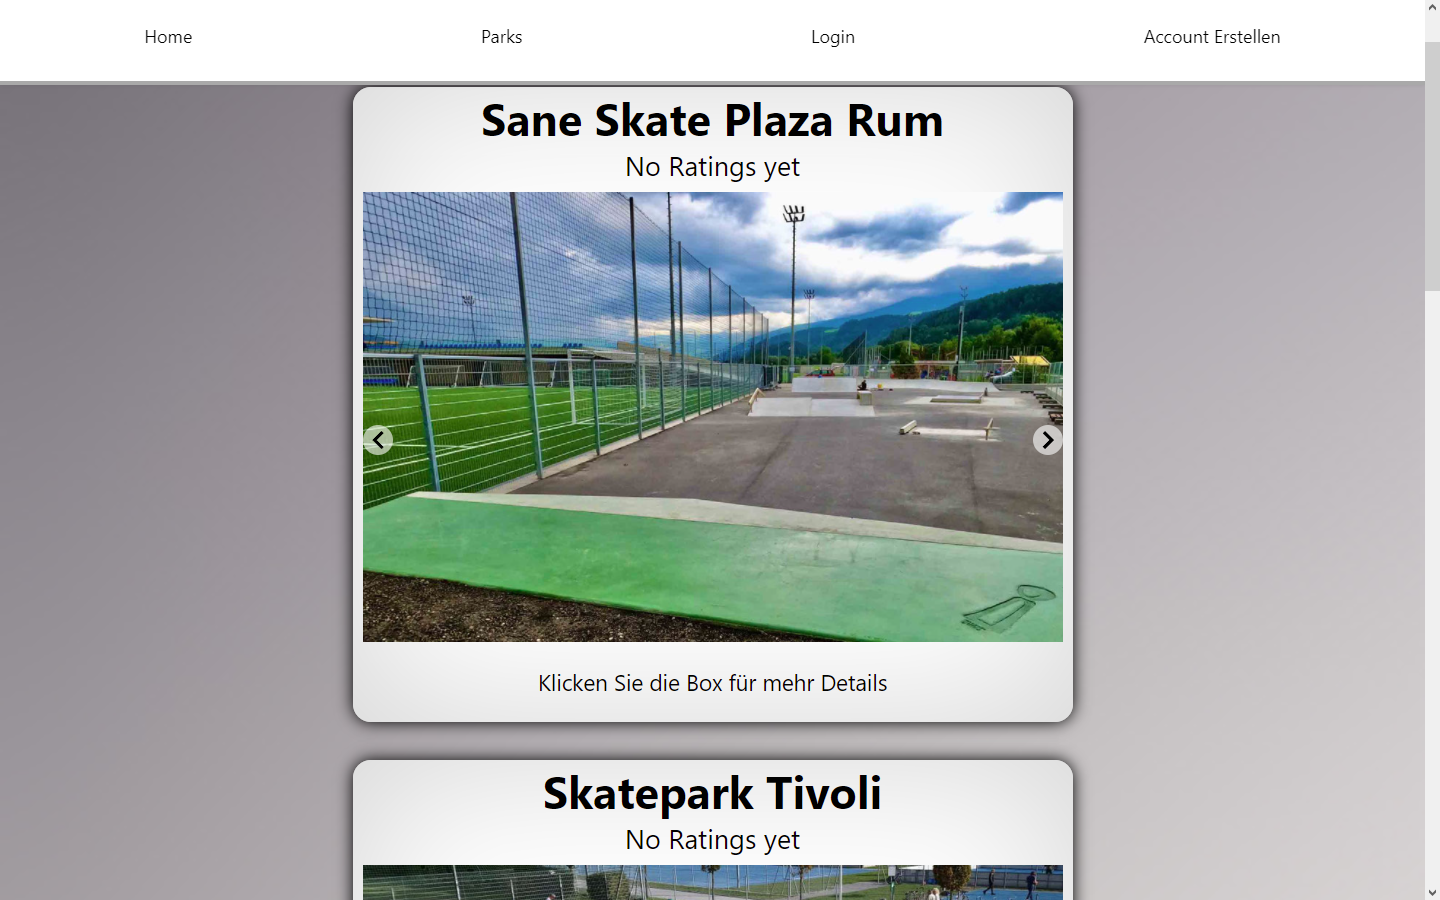
\includegraphics[width=1\textwidth]{Website/Parkliste.png}}
      \caption{Liste der Parks}
    \end{center}
\end{figure}

Hier wurde die selbe \nameref{slideshow} verwendet wie auf der Startseite. Wird ein Mausklick auf die 
Boxen betätigt, gelangt der Benutzer auf die \nameref{parkDetails} des Parks, wo die Bewertungen und Hindernisse,
welche der Park besitzt zu finden sind. 

\subsection{Suchleiste}

Ganz oben auf der Parklisten Ansicht befindet sich eine Suchleiste, welche zum Finden von Parks dient.

\begin{figure}[H]
    \begin{center}
      \frame{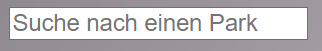
\includegraphics[width=0.5\textwidth]{Website/Suchleiste.png}}
      \caption{Liste der Parks}
    \end{center}
\end{figure}

Wird in die Suchleiste eine Zeichenkette eingegeben, werden nur noch die Parks angezeigt, welche diese 
Zeichenkette in ihrem Namen beinhalten. Dabei wird Groß- und Kleinschreibung komplett ignoriert um ein 
leichteres Suchen zu ermöglichen. Dafür wird der Input ganz einfach bevor er mit den Namen verglichen wird 
auf Kleinbuchstaben umgeändert.


Ist ein Benutzer eingeloggt, befindet sich über der Suchleiste ein Knopf bei welchen es möglich ist Vorschläge
zu erstellen.